\documentclass[12pt,a4paper,preprint]{elsarticle}
\usepackage[T2A]{fontenc}
\usepackage[utf8]{inputenc}
\usepackage[russian]{babel}
\usepackage[a4paper,left=2cm,right=2cm,top=2cm,bottom=2.7cm]{geometry}
\usepackage{amsmath,amssymb,amsfonts,amsthm,bm,graphicx,booktabs,multirow,array,tabularx,xcolor,hyperref}

\makeatletter
\def\ps@pprintTitle{%
    \let\@mkboth\markboth
    \def\@evenhead{%
        \ifnum\c@page>1
            {\footnotesize\thepage}\hfil{\footnotesize\itshape\leftmark}%
        \fi}%
    \def\@oddfoot{\footnotesize\itshape
        Preprint, \today\hfill\thepage\relax}%
    \let\@evenfoot\@oddfoot
}
\AtBeginDocument{\pagestyle{pprintTitle}}
\makeatother
\graphicspath{{figs/}}

\begin{document}

\begin{frontmatter}

\title{Акустическая геометрия и динамика звуковых лучей\\
в релятивистской сферической аккреции}

\author{Alexander V. Semyannikov}
\address{Independent Researcher \\ \textit{Email: avsemyannikov@gmail.com}}

\begin{abstract}
В аналоговой гравитации звуковые волны в движущейся жидкости распространяются по нулевым геодезическим эффективной искривлённой метрики, что даёт контролируемую постановку для изучения физики горизонтов в астрофизической аккреции. Релятивистская акустическая метрика для сферической аккреции хорошо известна и использовалась в исследованиях устойчивости и квазинормальных мод, однако геометрической оптике звуковых лучей в течении Мишеля до сих пор уделялось мало систематического внимания. В настоящей работе строится акустическая метрика идеальной жидкости, аккрецирующей на чёрную дыру Шварцшильда (течение Мишеля), и рассматриваются высокочастотные звуковые лучи как её нулевые геодезические. Из линеаризованной системы уравнений непрерывности, Эйлера и энергии выделяются причинные поверхности геометрии --- акустический горизонт (совпадающий со звуковой точкой), поверхность стационарного предела и эргообласть --- и выводится обобщённое уравнение Бине, разделяющее отклонение луча на вклады Эйнштейна, рефракции и акустического ветра. Фактор локального замедления позволяет сравнить акустическую и вакуумную задержки Шапиро, локализовать акустическую фотонную сферу и связать аналоговый масштаб Хокинга с гидродинамическими градиентами. Результаты для политропных индексов $\gamma=4/3$ и $5/3$ показывают, как термодинамические параметры и параметры потока аккреции входят в акустическое линзирование, временную задержку и аналоговую температуру Хокинга, формируя геометрическую основу для будущих исследований акустических, вихревых и энтропийных мод конечной частоты.
\end{abstract}

\begin{keyword}
акустическая метрика \sep аналоговая гравитация \sep аккреция Мишеля \sep
задержка Шапиро \sep звуковые лучи \sep акустический горизонт \sep фотонная сфера \sep
температура Хокинга
\end{keyword}

\end{frontmatter}

\section{Введение}
\label{sec:introduction}

Аккреция на чёрные дыры представляет собой центральный процесс в астрофизике высоких энергий: поток вещества на компактный объект формирует электромагнитное излучение, питает активные ядра галактик и обеспечивает одну из немногих лабораторий, в которых сильная гравитация может исследоваться наблюдательно~\cite{ShapiroSL_TeukolskySA_BlackHolesWhiteDwarfsAndNeutronStarsThePhysicsOfCompactObjects_2004}. Наряду с геометрией самого пространства-времени, \emph{гидродинамика} аккрецирующей жидкости поддерживает независимую причинную структуру для звука. В движущейся среде акустические возмущения распространяются так, как если бы они существовали на эффективной лоренцевой геометрии --- \emph{акустической метрике}, --- чьи нулевые конусы определяют звуковые горизонты, эргообласти и, в подходящих режимах, аналоги излучения Хокинга~\cite{UnruhWG_ExperimentalBlackHoleEvaporation_1981, VisserM_AcousticBlackHolesHorizonsErgospheresAndHawkingRadiation_1998, BarceloC_LiberatiS_VisserM_AnalogueGravity_2011}. Данное соответствие аналоговой гравитации связывает теорию волновых уравнений в искривлённом пространстве-времени и астрофизику трансзвуковой аккреции.

Классическое ньютоново описание стационарной сферической аккреции принадлежит Бонди~\cite{BondiH_OnSphericallySymmetricalAccretion_1953}. Его общерелятивистский аналог на фоне Шварцшильда --- течение Мишеля~\cite{MichelFC_AccretionOfMatterByCondensedObjects_1972} --- представляет собой стационарное, сферически симметричное, адиабатическое решение, проходящее через звуковую точку и становящееся сверхзвуковым вблизи горизонта событий. Линейные акустические возмущения таких течений описываются скалярным волновым уравнением на эффективной метрике, построенной из фонового пространства-времени, 4-скорости жидкости и локальной скорости звука. Версия этой конструкции присутствует в анализе Монкрифа устойчивости сферической аккреции на чёрную дыру Шварцшильда~\cite{MoncriefV_StabilityOfStationarySphericalAccretionOntoASchwarzschildBlackHole_1980}; релятивистская акустическая геометрия была систематизирована Биличем~\cite{BilicN_RelativisticAcousticGeometry_1999} и помещена в более широкий контекст аналоговой гравитации Виссером~\cite{VisserM_AcousticBlackHolesHorizonsErgospheresAndHawkingRadiation_1998}, а также Барсело, Либерати и Виссером~\cite{BarceloC_LiberatiS_VisserM_AnalogueGravity_2011}.

В указанной постановке значительная часть работ по аккреции Мишеля сосредоточена на волновом уравнении: глобальной устойчивости вне звукового горизонта, энергетических оценках и спектре квазинормальных акустических колебаний~\cite{MoncriefV_StabilityOfStationarySphericalAccretionOntoASchwarzschildBlackHole_1980, ChaverraE_MoralesMD_SarbachO_QuasinormalAcousticOscillationsInTheMichelFlow_2015}, а аналоговое излучение Хокинга переосмыслено как процесс туннелирования~\cite{JangidN_RayAK_AcousticHawkingRadiationAsATunnellingEffectInMichelAccretion_2026}. Комплементарная линия работ выражает акустическую поверхностную гравитацию и аналоговую температуру Хокинга непосредственно через переменные аккреции для релятивистских течений~\cite{DasTK_BilicN_DasguptaS_BlackHoleAccretionDiscAsAnAnalogueGravityModel_2007, TarafdarP_DasTK_GeometricConfigurationOfMatterForAxiallySymmetricBackgroundFlowsInTheSchwarzschildMetric_2013, ShaikhMA_FirdousiI_DasTK_RelativisticSonicGeometryForIsothermalAccretionInTheSchwarzschildMetric_2017}. Лучевые свойства акустических метрик изучались преимущественно в других аналоговых постановках~\cite{ToshmatovB_AhmedovB_StuchlikZ_PhononMotionAround21DimensionalAcousticBlackHole_2023, BalaliAE_MarraniA_LenseThirringAcousticBlackHolesShadowsAndLight_2025, VieiraHS_DestounisK_KokkotasKD_AnalogSchwarzschildBlackHolesOfBoseEinsteinCondensatesInACavityQuasinormalModesAndQuasiboundStates_2023, PalK_PalK_SarkarT_AnalogueMetricInABlackBounceBackground_2022}. Перечисленные исследования устанавливают акустическую геометрию аккреции Мишеля как подлинную астрофизическую аналоговую чёрную дыру, однако не формируют единой геометрико-оптической феноменологии \emph{звуковых лучей} для релятивистского адиабатического течения.

В вакуумной теории нулевые геодезические лежат в основе гравитационного линзирования, фотонной сферы и временной задержки Шапиро~\cite{ShapiroII_FourthTestOfGeneralRelativity_1964}. Для релятивистской аккреции Мишеля данные вопросы на уровне лучей --- силы, отклоняющие звуковой луч, акустическая задержка Шапиро, смещение акустической фотонной сферы и поверхностная гравитация звукового горизонта --- до настоящего времени не были сведены в единую количественную картину, связанную с термодинамикой потока.

В настоящей работе строится релятивистская акустическая метрика идеальной жидкости в стационарной аккреции Мишеля на чёрную дыру Шварцшильда и изучаются её высокочастотные звуковые лучи как нулевые геодезические эффективного пространства-времени. А именно:
\begin{itemize}
    \item определяются акустический горизонт, поверхность стационарного предела и эргообласть, проверяется совпадение горизонта со звуковой точкой Мишеля;
    \item выводится обобщённое уравнение Бине, разлагающее отклонение луча на силы Эйнштейна, рефракции и акустического ветра, численно оцениваются данные вклады для политропных индексов $\gamma=4/3$ и $5/3$;
    \item вводится фактор локального замедления $n_{\pm}=f/|v_{\pm}|$ и используется для сравнения акустической и вакуумной задержек Шапиро вдоль радиальных лучей;
    \item локализуется акустическая фотонная сфера, описывается связанный с ней барьер захвата и выражается поверхностная гравитация звукового горизонта через гидродинамические градиенты.
\end{itemize}

\section{Релятивистская жидкость и акустические возмущения}
\label{sec:fluid}

Термодинамические и гидродинамические элементы, необходимые для определения акустической метрики, резюмируются ниже. На протяжении работы используется сигнатура метрики $\mathfrak{s}=(-,+,+,+)$, так что 4-скорость жидкости удовлетворяет условию
\begin{equation}
    u_{\mu} u^{\mu} = -1.
    \label{eq:four-velocity-norm}
\end{equation}
Все величины безразмерны: пространственно-временные координаты измеряются в единицах гравитационного радиуса $r_{\mathrm{g}}=2GM/c^{2}$, 4-скорость и скорость звука --- в единицах $c$, а термодинамические переменные нормированы на свои асимптотические покоящиеся масштабы~\cite{MichelFC_AccretionOfMatterByCondensedObjects_1972, MoncriefV_StabilityOfStationarySphericalAccretionOntoASchwarzschildBlackHole_1980}. Ортогональные проекции на систему покоя жидкости выполняются с помощью
\begin{equation}
    \Delta^{\mu}_{\nu} = \delta^{\mu}_{\nu} + u^{\mu} u_{\nu}.
    \label{eq:projection-tensor}
\end{equation}

\subsection{Термодинамика идеальной жидкости}

Среда моделируется как идеальная жидкость в локальном термодинамическом равновесии. Безразмерная удельная энтальпия определяется как
\begin{equation}
    h = \frac{p + \epsilon}{n},
    \label{eq:specific-enthalpy}
\end{equation}
где $p$, $\epsilon$ и $n$ --- безразмерные давление, плотность энергии и барионная плотность числа частиц. Первое начало термодинамики,
\begin{equation}
    \mathrm{d}h = T\,\mathrm{d}S + n^{-1}\,\mathrm{d}p,
    \label{eq:first-law-thermodynamics}
\end{equation}
для адиабатического течения ($S=\mathrm{const}$) сводится к
\begin{equation}
    \mathrm{d}p = n\,\mathrm{d}h.
    \label{eq:adiabatic-relation}
\end{equation}
Совместно с~\eqref{eq:specific-enthalpy} это даёт тождество $\mathrm{d}\epsilon = h\,\mathrm{d}n$: в адиабатическом процессе изменение плотности энергии обусловлено исключительно изменением плотности частиц.

Локальная скорость звука задаётся изэнтропической производной
\begin{equation}
    a^{2}
    =
    \Bigl(\frac{\partial p}{\partial\epsilon}\Bigr)_{S}
    =
    \frac{1}{h}\,\frac{\mathrm{d}p}{\mathrm{d}n}.
    \label{eq:sound-speed-def}
\end{equation}
Термодинамика замыкается политропным уравнением состояния $p = K n^{\gamma}$. Интегрирование~\eqref{eq:adiabatic-relation} приводит к
\begin{equation}
    h = 1 + \frac{\gamma K}{\gamma-1}\, n^{\gamma-1},
    \label{eq:enthalpy-polytropic}
\end{equation}
а подстановка в~\eqref{eq:sound-speed-def} даёт
\begin{equation}
    a^{2}
    =
    \frac{K\gamma\, n^{\gamma-1}}
         {1 + \dfrac{\gamma K}{\gamma-1}\, n^{\gamma-1}}.
    \label{eq:sound-speed-polytropic}
\end{equation}
В холодном нерелятивистском пределе $h\to 1$ восстанавливается ньютоново соотношение $a^{2}\approx K\gamma n^{\gamma-1}$. В ультрарелятивистском пределе $n\to\infty$ возникает универсальная граница $a^{2}\to\gamma-1$; причинность ($a^{2}\le 1$) требует $\gamma\le 2$.

Для дальнейшего использования записывается конформный фактор акустической метрики, выраженный через локальную скорость звука:
\begin{equation}
    \Omega^{2} 
    = \frac{n}{h} 
    \quad\Longrightarrow\quad \Omega^{2}
    = C\, a^{\frac{2}{\gamma-1}}
    \Biggl(
        \frac{\gamma-1}{\gamma-1-a^{2}}
    \Biggr)^{\frac{2-\gamma}{\gamma-1}},
    \label{eq:conformal-factor}
\end{equation}
где $C=(K\gamma)^{-1/(\gamma-1)}$ фиксируется энтропией потока. Глобальная константа $C$ сокращается в условии нулевого интервала и не влияет на кинематику звуковых лучей.

\subsection{Уравнения гидродинамики}

Сохранение числа частиц выражается уравнением непрерывности
\begin{equation}
    \nabla_{\mu}\bigl(n\, u^{\mu}\bigr) = 0.
    \label{eq:continuity-equation}
\end{equation}
Ковариантное сохранение тензора энергии-импульса идеальной жидкости,
\begin{equation}
    T^{\mu}_{\nu} = nh\, u^{\mu} u_{\nu} + p\,\delta^{\mu}_{\nu},
    \qquad
    \nabla_{\mu} T^{\mu}_{\nu} = 0,
    \label{eq:stress-energy-tensor}
\end{equation}
вместе с~\eqref{eq:continuity-equation} и~\eqref{eq:adiabatic-relation} приводит к релятивистскому уравнению Эйлера
\begin{equation}
    h\, u^{\mu}\nabla_{\mu} u_{\nu}
    +
    \Delta^{\mu}_{\nu}\nabla_{\mu} h
    = 0.
    \label{eq:euler-enthalpy}
\end{equation}
Вводя релятивистскую 2-форму завихрённости
\begin{equation}
    \omega_{\mu\nu}
    \equiv
    \partial_{\mu}\bigl(h u_{\nu}\bigr)
    -
    \partial_{\nu}\bigl(h u_{\mu}\bigr)
    \label{eq:vorticity-2form}
\end{equation}
и допуская ненулевой градиент энтропии, уравнение~\eqref{eq:euler-enthalpy} переписывается в форме Лихнеровича--Крокко:
\begin{equation}
    u^{\mu}\omega_{\mu\nu} = T\,\partial_{\nu} S.
    \label{eq:euler-vorticity}
\end{equation}
Проекция $\nabla_{\mu}T^{\mu}_{\nu}=0$ вдоль потока эквивалентна адвекции энтропии,
\begin{equation}
    u^{\mu}\partial_{\mu} S = 0.
    \label{eq:entropy-advection}
\end{equation}
Триада~\eqref{eq:continuity-equation}--\eqref{eq:euler-vorticity}--\eqref{eq:entropy-advection} замыкает динамику идеальной жидкости. При линеаризации она разбивает спектр возмущений на три семейства: акустические, вихревые и энтропийные моды~\cite{MoncriefV_StabilityOfStationarySphericalAccretionOntoASchwarzschildBlackHole_1980}.

\subsection{Линейные возмущения и акустическое волновое уравнение}

Каждое поле представляется в виде фонового значения и поправки первого порядка,
\begin{equation}
    h\to h+\delta h,\quad
    u^{\mu}\to u^{\mu}+\delta u^{\mu},\quad
    n\to n+\delta n,\quad
    S\to S+\delta S.
    \label{eq:perturbation-expansion}
\end{equation}
Возмущения плотности и энтальпии связаны соотношением
\begin{equation}
    \delta n = \frac{n}{a^{2} h}\,\delta h,
    \label{eq:density-enthalpy-perturbation}
\end{equation}
а линеаризация~\eqref{eq:four-velocity-norm} накладывает условие ортогональности $u_{\mu}\delta u^{\mu}=0$. Линеаризованное уравнение непрерывности принимает вид
\begin{equation}
    \nabla_{\mu}
    \Biggl(
        n
        \Biggl[
            \delta u^{\mu}
            +
            \frac{u^{\mu}}{h a^{2}}\,\delta h
        \Biggr]
    \Biggr)
    = 0.
    \label{eq:linearized-continuity}
\end{equation}

Фон полагается гомоэнтропическим ($\nabla_{\mu}S=0$) и безвихревым ($\omega_{\mu\nu}=0$). Определяя возмущённый обобщённый импульс
\begin{equation}
    w_{\mu}
    \equiv
    \delta\bigl(h u_{\mu}\bigr)
    =
    h\,\delta u_{\mu} + u_{\mu}\,\delta h
    \label{eq:perturbed-momentum}
\end{equation}
и его завихрённость $\delta\omega_{\mu\nu}=\partial_{\mu}w_{\nu}-\partial_{\nu}w_{\mu}$, линеаризованное уравнение Эйлера записывается как
\begin{equation}
    u^{\mu}\,\delta\omega_{\mu\nu} = T\,\partial_{\nu}\delta S.
    \label{eq:linearized-euler}
\end{equation}
Для акустических мод ($\delta S=0$, $\delta\omega_{\mu\nu}=0$) выполняется $w_{\mu}=\partial_{\mu}\delta\psi$, что выражает гидродинамические поля через скалярный потенциал:
\begin{equation}
    h\,\delta u_{\mu} + u_{\mu}\,\delta h = \partial_{\mu}\delta\psi.
    \label{eq:velocity-potential-def}
\end{equation}
Свёртка с $u^{\mu}$ даёт
\begin{equation}
    \delta h = -\,u^{\mu}\partial_{\mu}\delta\psi,
    \label{eq:enthalpy-potential-relation}
\end{equation}
а проектор~\eqref{eq:projection-tensor} приводит к
\begin{equation}
    h\,\delta u_{\mu}
    =
    \Delta^{\nu}_{\mu}\,\partial_{\nu}\delta\psi.
    \label{eq:velocity-potential-gradient}
\end{equation}
Подстановка~\eqref{eq:enthalpy-potential-relation} и~\eqref{eq:velocity-potential-gradient} в~\eqref{eq:linearized-continuity} даёт волновое уравнение
\begin{equation}
    \nabla_{\mu}\bigl(\mathcal{G}^{\mu\nu}\partial_{\nu}\delta\psi\bigr) = 0,
    \label{eq:wave-equation}
\end{equation}
в котором контравариантная акустическая метрика имеет вид
\begin{equation}
    \mathcal{G}^{\mu\nu} = \Omega^{2}\,\eta^{\mu\nu},
    \qquad
    \eta^{\mu\nu} = g^{\mu\nu} + \alpha\, u^{\mu} u^{\nu},
    \label{eq:acoustic-metric-tensor}
\end{equation}
с параметром увлечения $\alpha=1-a^{-2}$. Ковариантный аналог записывается как
\begin{equation}
    \mathcal{G}_{\mu\nu} = \Omega^{-2}\,\eta_{\mu\nu},
    \qquad
    \eta_{\mu\nu} = g_{\mu\nu} - \beta\, u_{\mu} u_{\nu},
    \label{eq:covariant-acoustic-metric-tensor}
\end{equation}
где $\beta = a^{2}-1$. Конструкция~\eqref{eq:acoustic-metric-tensor}--\eqref{eq:covariant-acoustic-metric-tensor} представляет собой релятивистскую акустическую геометрию Билича~\cite{BilicN_RelativisticAcousticGeometry_1999}. Высокочастотные звуковые лучи являются нулевыми геодезическими $\mathcal{G}_{\mu\nu}$.

\section{Акустическая геометрия аккреции Мишеля}
\label{sec:acoustic-geometry}

Акустическая метрика специализируется на стационарную, сферически симметричную, адиабатическую аккрецию на чёрную дыру Шварцшильда --- течение Мишеля~\cite{MichelFC_AccretionOfMatterByCondensedObjects_1972}.

\subsection{Фоновое пространство-время Шварцшильда}

Фоновый интервал записывается в виде
\begin{equation}
    \mathrm{d}s^{2}
    =
    -f\,\mathrm{d}t^{2}
    +
    f^{-1}\,\mathrm{d}r^{2}
    +
    r^{2}\bigl(\mathrm{d}\theta^{2}+\sin^{2}\!\theta\,\mathrm{d}\phi^{2}\bigr),
    \label{eq:schwarzschild-metric}
\end{equation}
с безразмерной lapse-функцией
\begin{equation}
    f = 1 - r^{-1}.
    \label{eq:lapse-function}
\end{equation}
В матричной записи
\begin{equation}
    g^{\mu\nu}
    =
    \begin{pmatrix}
        -f^{-1} & 0 & 0 & 0 \\
        0 & f & 0 & 0 \\
        0 & 0 & r^{-2} & 0 \\
        0 & 0 & 0 & r^{-2}\sin^{-2}\!\theta
    \end{pmatrix},
    \qquad
    g_{\mu\nu}
    =
    \begin{pmatrix}
        -f & 0 & 0 & 0 \\
        0 & f^{-1} & 0 & 0 \\
        0 & 0 & r^{2} & 0 \\
        0 & 0 & 0 & r^{2}\sin^{2}\!\theta
    \end{pmatrix}.
    \label{eq:schwarzschild-metric-matrix}
\end{equation}
В силу стационарности и сферической симметрии каждый фоновый скаляр зависит только от $r$. При записи
\begin{equation}
    u^{\mu} = (\vartheta,\,\upsilon,\,0,\,0),
    \label{eq:four-velocity-schwarzschild}
\end{equation}
получаются ковариантные компоненты $u_{\mu}=(-f\vartheta,\,f^{-1}\upsilon,\,0,\,0)$, а нормировка~\eqref{eq:four-velocity-norm} принимает вид
\begin{equation}
    -u_{t} = f\vartheta = \sqrt{f+\upsilon^{2}},
    \label{eq:four-velocity-norm-schwarzschild}
\end{equation}
связывая временную компоненту с радиальной 3-скоростью потока. Физическая скорость, измеряемая статическим наблюдателем,
\begin{equation}
    V = \frac{|\upsilon|}{\sqrt{f+\upsilon^{2}}},
    \label{eq:physical-velocity}
\end{equation}
входит в число Маха $\mathcal{M}=V/a$.

Фон Мишеля фиксируется двумя интегралами движения: непрерывность даёт барионный поток $r^{2} n\,\upsilon=\mathrm{const}$ ($\upsilon<0$ при аккреции), а адиабатическая проекция интегрируется в релятивистский интеграл Бернулли
\begin{equation}
    h\sqrt{f+\upsilon^{2}} = h_{\infty}.
    \label{eq:michel-bernoulli}
\end{equation}
Совместно с политропным замыканием данные соотношения определяют профили $\upsilon(r)$, $a(r)$ и $n(r)$~\cite{MichelFC_AccretionOfMatterByCondensedObjects_1972, ShapiroSL_TeukolskySA_BlackHolesWhiteDwarfsAndNeutronStarsThePhysicsOfCompactObjects_2004}.

\subsection{Акустический метрический тензор}

Подстановка~\eqref{eq:schwarzschild-metric-matrix} и~\eqref{eq:four-velocity-schwarzschild} в ковариантное ядро~\eqref{eq:covariant-acoustic-metric-tensor} приводит к
\begin{equation}
    \eta_{\mu\nu}
    =
    \begin{pmatrix}
        -f\bigl(1+\beta f\vartheta^{2}\bigr) &
        \beta\vartheta\upsilon & 0 & 0 \\
        \beta\vartheta\upsilon &
        f^{-1}\bigl(1-\beta f^{-1}\upsilon^{2}\bigr) & 0 & 0 \\
        0 & 0 & r^{2} & 0 \\
        0 & 0 & 0 & r^{2}\sin^{2}\!\theta
    \end{pmatrix}.
    \label{eq:eta-covariant-matrix}
\end{equation}
Полная ковариантная акустическая метрика определяется как $\mathcal{G}_{\mu\nu}=\Omega^{-2}\eta_{\mu\nu}$. Соответствующее контравариантное ядро записывается в виде
\begin{equation}
    \eta^{\mu\nu}
    =
    \begin{pmatrix}
        -f^{-1}+\alpha\vartheta^{2} &
        \alpha\vartheta\upsilon & 0 & 0 \\
        \alpha\vartheta\upsilon &
        f+\alpha\upsilon^{2} & 0 & 0 \\
        0 & 0 & r^{-2} & 0 \\
        0 & 0 & 0 & r^{-2}\sin^{-2}\!\theta
    \end{pmatrix}.
    \label{eq:eta-contravariant-matrix}
\end{equation}
Поскольку звуковые лучи являются нулевыми геодезическими $\mathcal{G}_{\mu\nu}$, они инвариантны относительно конформных перемасштабирований:
\begin{equation}
    \mathcal{G}_{\mu\nu}k^{\mu}k^{\nu}=0 \quad\Longrightarrow\quad \eta_{\mu\nu}k^{\mu}k^{\nu} = 0.
    \label{eq:acoustic-null-condition}
\end{equation}
Геометрия акустического светового конуса полностью фиксируется ядром $\eta_{\mu\nu}$.

\subsection{Акустический горизонт, стационарный предел и эргообласть}

Акустический горизонт событий $r=r_{\mathrm{a}}$ представляет собой одностороннюю мембрану для звука и формируется там, где поток становится звуковым или сверхзвуковым, что эквивалентно обращению в нуль радиальной компоненты ядра:
\begin{equation}
    \eta^{rr}(r_{\mathrm{a}}) = 0
    \quad\Longrightarrow\quad
    r_{\mathrm{a}}
    =
    \bigl[1 + \alpha(r_{\mathrm{a}})\,\upsilon^{2}(r_{\mathrm{a}})\bigr]^{-1}.
    \label{eq:acoustic-horizon-def}
\end{equation}
При $r<r_{\mathrm{a}}$ все характеристики волнового уравнения направлены внутрь.

Поверхность акустического стационарного предела $r=r_{\mathrm{asl}}$ определяется обращением в нуль временной компоненты ядра,
\begin{equation}
    \eta^{tt}(r_{\mathrm{asl}}) = 0
    \quad\Longrightarrow\quad
    r_{\mathrm{asl}}
    =
    \frac{\alpha(r_{\mathrm{asl}})\,\vartheta^{2}(r_{\mathrm{asl}})}
         {\alpha(r_{\mathrm{asl}})\,\vartheta^{2}(r_{\mathrm{asl}})-1}.
    \label{eq:stationary-limit-def}
\end{equation}
Внутри $r<r_{\mathrm{asl}}$ стационарная акустическая мода существовать не может. Приравнивание~\eqref{eq:acoustic-horizon-def} и~\eqref{eq:stationary-limit-def} потребовало бы $a^{2}<0$, что невозможно для устойчивой среды. Следовательно, две поверхности никогда не совпадают, $r_{\mathrm{a}} \neq r_{\mathrm{asl}}$, а конечная оболочка между ними составляет акустическую эргообласть~\cite{VisserM_AcousticBlackHolesHorizonsErgospheresAndHawkingRadiation_1998, BilicN_RelativisticAcousticGeometry_1999}.

Ключевым структурным фактом аккреции Мишеля является точное совпадение акустического горизонта со звуковой критической точкой фонового течения. Гладкий трансзвуковой переход через $r=r_{\mathrm{c}}$ требует одновременного обращения в нуль числителя и знаменателя уравнения для радиального градиента~\cite{ShapiroSL_TeukolskySA_BlackHolesWhiteDwarfsAndNeutronStarsThePhysicsOfCompactObjects_2004}, что приводит к стандартным условиям критической точки:
\begin{equation}
    \upsilon^{2}_{\mathrm{c}} = \frac{1}{4r_{\mathrm{c}}},
    \qquad
    a^{2}_{\mathrm{c}}
    =
    \frac{1}{4r_{\mathrm{c}}-3}
    =
    \frac{\upsilon^{2}_{\mathrm{c}}}{1-3\upsilon^{2}_{\mathrm{c}}}.
    \label{eq:michel-sonic}
\end{equation}
Подстановка данных значений в $\eta^{rr}$ из~\eqref{eq:eta-contravariant-matrix} даёт
\begin{equation}
    1 - a^{-2}_{\mathrm{c}}
    =
    4(1-r_{\mathrm{c}}),
    \qquad
    \bigl(1-a^{-2}_{\mathrm{c}}\bigr)\upsilon^{2}_{\mathrm{c}}
    =
    -f_{\mathrm{c}},
\end{equation}
в результате чего
\begin{equation}
    \eta^{rr}(r_{\mathrm{c}}) = f_{\mathrm{c}} - f_{\mathrm{c}} = 0.
    \label{eq:sonic-is-horizon}
\end{equation}
Следовательно, $r_{\mathrm{a}}=r_{\mathrm{c}}$: поверхность, на которой аккреционный поток становится звуковым, \emph{является} акустическим горизонтом событий. Оболочка $1<r<r_{\mathrm{a}}$ сверхзвуковая ($\eta^{rr}<0$) и заканчивается на гравитационном горизонте $r=1$.

Интеграл Бернулли~\eqref{eq:michel-bernoulli} связывает $a_{\infty}$ с радиусом горизонта $r_{\mathrm{a}}$; типичные значения представлены в табл.~\ref{tab:sonic-point}. Численные результаты опираются на фоновые профили, которые находятся путём интегрирования внутрь от большого радиуса. Акустическая фотонная сфера $r_{\mathrm{aph}}$ находится как максимум барьера захвата $U(r)=a^{2}\eta^{rr}/r^{2}$.

\section{Динамика звуковых лучей}
\label{sec:rays}

В высокочастотном пределе акустические возмущения распространяются вдоль нулевых геодезических $\mathcal{G}_{\mu\nu}$, представляющих собой акустический аналог световых лучей в вакууме~\cite{VisserM_AcousticBlackHolesHorizonsErgospheresAndHawkingRadiation_1998, BarceloC_LiberatiS_VisserM_AnalogueGravity_2011}.

\subsection{Нулевые геодезические и сохраняющиеся величины}

Стационарность и сферическая симметрия фона Мишеля обеспечивают наличие двух векторов Киллинга $\partial_{t}$ и $\partial_{\phi}$, которые наделяют каждый звуковой луч сохраняющимися энергией и угловым моментом. Сами лучи представляют собой нулевые геодезические акустической метрики,
\begin{equation}
    \frac{\mathrm{d}^{2}x^{\mu}}{\mathrm{d}\lambda^{2}}
    +
    \Gamma^{\mu}_{\alpha\beta}
    \frac{\mathrm{d}x^{\alpha}}{\mathrm{d}\lambda}
    \frac{\mathrm{d}x^{\beta}}{\mathrm{d}\lambda}
    = 0,
    \label{eq:geodesic-equation}
\end{equation}
с волновым вектором $k^{\mu}=\mathrm{d}x^{\mu}/\mathrm{d}\lambda$. Стационарность $\mathcal{G}_{\mu\nu}$ даёт сохраняющуюся по Киллингу энергию
\begin{equation}
    k_{t} = \mathcal{G}_{t\mu}k^{\mu} = -E = \mathrm{const},
    \label{eq:energy-conservation}
\end{equation}
где знак минус следует из сигнатуры~\eqref{eq:four-velocity-norm}. В силу того, что $\mathcal{G}_{rt}\neq 0$,
\begin{equation}
    \frac{\mathrm{d}t}{\mathrm{d}\lambda}
    =
    -\frac{1}{\mathcal{G}_{tt}}
    \Biggl(
        E + \mathcal{G}_{rt}\,\frac{\mathrm{d}r}{\mathrm{d}\lambda}
    \Biggr),
    \label{eq:time-coordinate-derivative}
\end{equation}
координатное время вдоль луча жёстко связано с его радиальным движением: втекающий поток увлекает луч вперёд по $t$, что служит акустическим аналогом увлечения систем отсчёта.

Второй вектор Киллинга, $\partial_{\phi}$, аналогичным образом сохраняет угловой момент. Ограничиваясь без потери общности экваториальной плоскостью $\theta=\pi/2$, получают
\begin{equation}
    k_{\phi} = \mathcal{G}_{\phi\phi}\,\frac{\mathrm{d}\phi}{\mathrm{d}\lambda} = L = \mathrm{const}.
    \label{eq:angular-momentum-conservation}
\end{equation}
Их отношение $b=L/E$ представляет собой прицельный параметр.

При фиксированных $E$ и $L$ условие нулевого интервала~\eqref{eq:acoustic-null-condition} сводится к уравнению для радиального движения,
\begin{equation}
    \mathcal{G}_{tt}\Biggl(\frac{\mathrm{d}t}{\mathrm{d}\lambda}\Biggr)^{2}
    +
    2\mathcal{G}_{tr}\,\frac{\mathrm{d}t}{\mathrm{d}\lambda}\,\frac{\mathrm{d}r}{\mathrm{d}\lambda}
    +
    \mathcal{G}_{rr}\Biggl(\frac{\mathrm{d}r}{\mathrm{d}\lambda}\Biggr)^{2}
    +
    \frac{L^{2}}{\mathcal{G}_{\phi\phi}}
    = 0.
    \label{eq:null-interval-expanded}
\end{equation}
Для радиальных лучей ($L=0$) оно сводится к квадратному уравнению для координатной скорости $v=\mathrm{d}r/\mathrm{d}t$,
\begin{equation}
    \mathcal{G}_{rr}v^{2} + 2\mathcal{G}_{rt}v + \mathcal{G}_{tt} = 0.
    \label{eq:coordinate-velocity-quadratic}
\end{equation}
При использовании~\eqref{eq:eta-covariant-matrix} и нормировки 4-скорости конформный фактор сокращается, а корни принимают вид
\begin{equation}
    v_{\pm}
    =
    \frac{-\beta\vartheta\upsilon \pm a}{f - \beta\upsilon^{2}}\, f^{2}.
    \label{eq:coordinate-velocity}
\end{equation}
Ветвь $v_{+}$ соответствует исходящему лучу, $v_{-}$ --- входящему. В вакуумном пределе $a\to 1$, $\beta\to 0$ восстанавливается $v_{\pm}=\pm f$. Акустический горизонт в точности совпадает с поверхностью вмораживания $v_{+}=0$, эквивалентной~\eqref{eq:acoustic-horizon-def}.

\subsection{Обобщённое уравнение Бине}

Нерадиальные лучи описываются как орбиты по углу $\phi$. При переходе к $\varrho=1/r$ и исключении аффинного параметра получается первый интеграл Бине:
\begin{equation}
    \Biggl(\frac{\mathrm{d}\varrho}{\mathrm{d}\phi}\Biggr)^{2}
    =
    \frac{1}{b^{2}a^{2}} - \varrho^{2}\eta^{rr}.
    \label{eq:binet-first-acoustic}
\end{equation}
Дифференцирование по $\phi$ приводит к уравнению Бине второго порядка:
\begin{equation}
    \frac{\mathrm{d}^{2}\varrho}{\mathrm{d}\phi^{2}} + \varrho
    =
    \underbrace{\vphantom{\frac{\mathrm{d}}{\mathrm{d}\varrho}\Bigl(\frac{1}{a^{2}}\Bigr)}\frac{3}{2}\varrho^{2}}_{F_{\mathrm{E}}}
    +
    \underbrace{\frac{1}{2b^{2}}\,\frac{\mathrm{d}}{\mathrm{d}\varrho}\!\Bigl(\frac{1}{a^{2}}\Bigr)}_{F_{\mathrm{R}}}
    -
    \underbrace{\vphantom{\frac{\mathrm{d}}{\mathrm{d}\varrho}\Bigl(\frac{1}{a^{2}}\Bigr)}\frac{1}{2}\,\frac{\mathrm{d}}{\mathrm{d}\varrho}\!\bigl(\alpha\upsilon^{2}\varrho^{2}\bigr)}_{F_{\mathrm{W}}}.
    \label{eq:binet-second-acoustic}
\end{equation}
В вакууме ($a\to 1$) данное уравнение сводится к стандартному шварцшильдовскому соотношению $\mathrm{d}^{2}\varrho/\mathrm{d}\phi^{2}+\varrho=\frac{3}{2}\varrho^{2}$. В общем случае правая часть распадается на три конкурирующие силы:
\begin{itemize}
    \item $F_{\mathrm{E}}$ --- отклонение Эйнштейна (вакуумная кривизна);
    \item $F_{\mathrm{R}}$ --- акустическая рефракция от градиентов $a(r)$;
    \item $F_{\mathrm{W}}$ --- сила акустического ветра от радиальной аккреции.
\end{itemize}
Численное интегрирование~\eqref{eq:binet-second-acoustic} для течения Мишеля при $a_{\infty}=0{,}1$ показывает, что лучи с $b<b_{\mathrm{c}}$ наматываются на акустический горизонт, тогда как лучи с $b>b_{\mathrm{c}}$ рассеиваются. Критический прицельный параметр $b_{\mathrm{c}}$ фиксируется максимумом барьера захвата
\begin{equation}
    U(r) = a^{2}\eta^{rr}/r^{2}
    \label{eq:capture-barrier}
\end{equation}
через условие поворота $1/b^{2}=U(r)$.

\subsection{Акустическая задержка Шапиро}

Помимо отклонения, звуковой луч характеризуется временной задержкой, представляющей собой акустический аналог эффекта Шапиро. Координатное время прохождения радиального луча между $r_{1}$ и $r_{2}$ определяется как
\begin{equation}
    t_{\pm}
    =
    \int^{r_{2}}_{r_{1}}\frac{\mathrm{d}r}{v_{\pm}(r)}
    =
    \int^{r_{2}}_{r_{1}}
    \frac{f-\beta\upsilon^{2}}{f^{2}\bigl(-\beta\vartheta\upsilon\pm a\bigr)}\,\mathrm{d}r.
    \label{eq:shapiro-time}
\end{equation}
В вакууме данное выражение сводится к классическому интегралу Шапиро~\cite{ShapiroII_FourthTestOfGeneralRelativity_1964}. В акустической геометрии возникают гидродинамическая и рефракционная задержки. Более чувствительным локальным индикатором выступает коэффициент замедления
\begin{equation}
    n_{\pm}(r) = \frac{f(r)}{|v_{\pm}(r)|},
    \label{eq:local-slowdown}
\end{equation}
показывающий, во сколько раз звуковой луч в данной точке медленнее вакуумного фотона. Вблизи горизонта исходящий луч замерзает ($v_{+}\to 0$, $n_{+}\to\infty$), а входящий сносится внутрь при конечном $n_{-}$.

Для исходящего сигнала избыточная задержка относительно плоского светового времени,
\begin{equation}
    \Delta t_{+}(r_{1})
    =
    \int^{r_{\mathrm{out}}}_{r_{1}}\frac{\mathrm{d}r}{v_{+}(r)} - \bigl(r_{\mathrm{out}}-r_{1}\bigr),
    \label{eq:shapiro-excess}
\end{equation}
превышает вакуумный аналог на множители $R=\Delta t^{\mathrm{ac}}_{+}/\Delta t^{\mathrm{vac}}_{+}\sim 10^{2}$--$10^{3}$.

\subsection{Акустическое линзирование и фотонная сфера}

Рассеиваемые лучи группируются вокруг единственной неустойчивой круговой орбиты --- акустической фотонной сферы $r_{\mathrm{aph}}$. В вакуумном пространстве-времени Шварцшильда эта орбита находится при $r_{\mathrm{ph}}=3/2$; в акустической геометрии условия круговой орбиты $\mathrm{d}\varrho/\mathrm{d}\phi=\mathrm{d}^{2}\varrho/\mathrm{d}\phi^{2}=0$ смещают её. Линеаризация в окрестности вакуумной точки $\varrho_{\mathrm{ph}}=2/3$ позволяет разделить сдвиг на рефракционный и ветровой вклады:
\begin{equation}
    \delta\varrho
    =
    \underbrace{\vphantom{\Biggl(
        \beta_{\mathrm{ph}}\upsilon^{2}_{\mathrm{ph}}
        +
        \frac{1}{3}\,\frac{\mathrm{d}(\beta\upsilon^{2})}{\mathrm{d}\varrho}\Big|_{\mathrm{ph}}
    \Biggr)}\frac{2}{27}\,\frac{\mathrm{d}\beta}{\mathrm{d}\varrho}\Big|_{\mathrm{ph}}}_{\delta F_{\mathrm{R}}}
    +
    \underbrace{\frac{2}{3}\Biggl(
        \beta_{\mathrm{ph}}\upsilon^{2}_{\mathrm{ph}}
        +
        \frac{1}{3}\,\frac{\mathrm{d}(\beta\upsilon^{2})}{\mathrm{d}\varrho}\Big|_{\mathrm{ph}}
    \Biggr)}_{-\delta F_{\mathrm{W}}},
    \label{eq:acoustic-photon-sphere-delta}
\end{equation}
в результате чего
\begin{equation}
    r_{\mathrm{aph}}
    \approx
    \frac{3}{2}\Biggl(1 - \frac{3}{2}\,\delta\varrho\Biggr).
    \label{eq:raph-from-delta}
\end{equation}
Для течения Мишеля при $a_{\infty}=0{,}1$ доминирует ветровой вклад, что приводит к существенному сдвигу наружу. Тень определяется радиусом $r_{\mathrm{aph}}$, а не самим горизонтом. Отношение $r_{\mathrm{aph}}/r_{\mathrm{a}}$ остаётся почти постоянным: $\approx 1{,}39$ для $\gamma=5/3$ и $\approx 1{,}42$ для $\gamma=4/3$.

\section{Поверхностная гравитация и аналоговая температура Хокинга}
\label{sec:surface-gravity}

Акустический горизонт $r=r_{\mathrm{a}}$ выступает необходимым кинематическим элементом для аналога излучения Хокинга. Темп экспоненциального растяжения исходящих нулевых лучей вблизи горизонта измеряется поверхностной гравитацией $\kappa$. На основе координатной скорости исходящего луча,
\begin{equation}
    v_{+}(r)
    =
    \frac{a - \beta\vartheta\upsilon}{f - \beta\upsilon^{2}}\, f^{2},
    \label{eq:v-plus}
\end{equation}
вводится акустическая черепашья координата $\mathrm{d}r_{*}=\mathrm{d}r/v_{+}(r)$. Вблизи горизонта $v_{+}(r)\approx (\mathrm{d}v_{+}/\mathrm{d}r)|_{r_{\mathrm{a}}}(r-r_{\mathrm{a}})$, в связи с чем
\begin{equation}
    r_{*}
    \approx
    \frac{1}{(\mathrm{d}v_{+}/\mathrm{d}r)|_{r_{\mathrm{a}}}}\,\ln(r-r_{\mathrm{a}}).
    \label{eq:tortoise-near-horizon}
\end{equation}
Сопоставление с канонической формой $r_{*}\sim(2\kappa)^{-1}\ln(r-r_{\mathrm{a}})$ приводит к инвариантному определению
\begin{equation}
    \kappa
    \equiv
    \frac{1}{2}\,\frac{\mathrm{d}v_{+}}{\mathrm{d}r}\Big|_{r=r_{\mathrm{a}}}.
    \label{eq:surface-gravity-def}
\end{equation}
Поскольку числитель~\eqref{eq:v-plus} на горизонте обращается в нуль, при дифференцировании сохраняется лишь производная данного числителя, что даёт замкнутое выражение:
\begin{equation}
    \kappa
    =
    \frac{f^{2}(r_{\mathrm{a}})}
         {2\bigl[f(r_{\mathrm{a}})-\beta(r_{\mathrm{a}})\upsilon^{2}(r_{\mathrm{a}})\bigr]}
    \,\frac{\mathrm{d}}{\mathrm{d}r}\bigl(a-\beta\vartheta\upsilon\bigr)\Big|_{r=r_{\mathrm{a}}}.
    \label{eq:surface-gravity-explicit}
\end{equation}
Поверхностная гравитация определяется \emph{скоростью} пересечения течением звуковой точки. Экспоненциальное красное смещение исходящих мод превращает асимптотический вакуум в тепловую ванну фононов с температурой
\begin{equation}
    T_{\mathrm{H}} = \frac{\kappa}{2\pi},
    \label{eq:hawking-temperature}
\end{equation}
или, при восстановлении размерности,
\begin{equation}
    k_{\mathrm{B}}T_{\mathrm{H}}
    =
    \frac{\hbar c}{2\pi r_{\mathrm{g}}}\,\kappa.
    \label{eq:hawking-temperature-dim}
\end{equation}
Относительно вакуумной поверхностной гравитации Шварцшильда $\kappa_{\mathrm{Sch}}=1/2$ отношение температур записывается как
\begin{equation}
    \frac{T^{\mathrm{ac}}_{\mathrm{H}}}{T^{\mathrm{vac}}_{\mathrm{H}}}
    =
    2\kappa(a,\vartheta,\upsilon).
    \label{eq:temperature-ratio}
\end{equation}
Горизонту также можно сопоставить формальную площадь в эффективной геометрии,
\begin{equation}
    \mathcal{A}_{\mathrm{a}}
    =
    \oint\sqrt{\mathcal{G}_{\theta\theta}\mathcal{G}_{\phi\phi}}\,\mathrm{d}\theta\,\mathrm{d}\phi
    =
    \frac{4\pi r^{2}_{\mathrm{a}}}{\Omega^{2}(r_{\mathrm{a}})},
    \label{eq:acoustic-horizon-area}
\end{equation}
однако акустический горизонт воспроизводит \emph{излучение} Хокинга как кинематический эффект, но не формирует полную термодинамику Бекенштейна---Хокинга.

\section{Заключение}

В настоящей работе построена релятивистская акустическая геометрия аккреции Мишеля идеальной жидкости на чёрную дыру Шварцшильда и проведён анализ высокочастотного звука как нулевых геодезических эффективной метрики $\mathcal{G}_{\mu\nu}$. На основе линеаризованной системы уравнений непрерывности, Эйлера и энергии показано, что волновое уравнение для потенциала скорости определяет $\mathcal{G}^{\mu\nu}=\Omega^{2}(g^{\mu\nu}+\alpha u^{\mu}u^{\nu})$ с $\alpha=1-a^{-2}$. На фоне Мишеля акустический горизонт событий в точности совпадает со звуковой критической точкой, $r_{\mathrm{a}}=r_{\mathrm{c}}$, тогда как поверхность стационарного предела остаётся отличной от него и ограничивает акустическую эргообласть.

Геометрическая оптика звуковых лучей описывается обобщённым уравнением Бине, разлагающим отклонение на силы Эйнштейна, рефракции и акустического ветра. Численное интегрирование при $a_{\infty}=0{,}1$ показывает, что вблизи горизонта доминирует ветер, рефракция на всём протяжении остаётся отталкивающей, а максимум барьера захвата фиксирует акустическую фотонную сферу, существенно смещённую наружу относительно вакуумного значения $r_{\mathrm{ph}}=3/2$. В диапазоне $a_{\infty}=0{,}05$--$0{,}20$ оба радиуса претерпевают сильные изменения, однако их отношение остаётся почти неизменным. Акустическая задержка Шапиро демонстрирует вмораживание исходящих лучей на горизонте и сходимость обеих ветвей к плато $1/a_{\infty}$ на больших радиусах.

Поверхностная гравитация на звуковом горизонте выражена через гидродинамические градиенты, благодаря чему аналоговая температура Хокинга зондирует скорость пересечения потоком звуковой точки. Естественным направлением дальнейших исследований выступает анализ пространственной устойчивости акустических, вихревых и энтропийных мод, требующий решения полного волнового уравнения с нетривиальным конформным фактором.

\section*{Благодарности}
В работе использована база данных NASA's Astrophysics Data System. Автор является независимым исследователем и выполнил эту работу без институционального финансирования.

\clearpage
\begin{figure}[p]
\centering
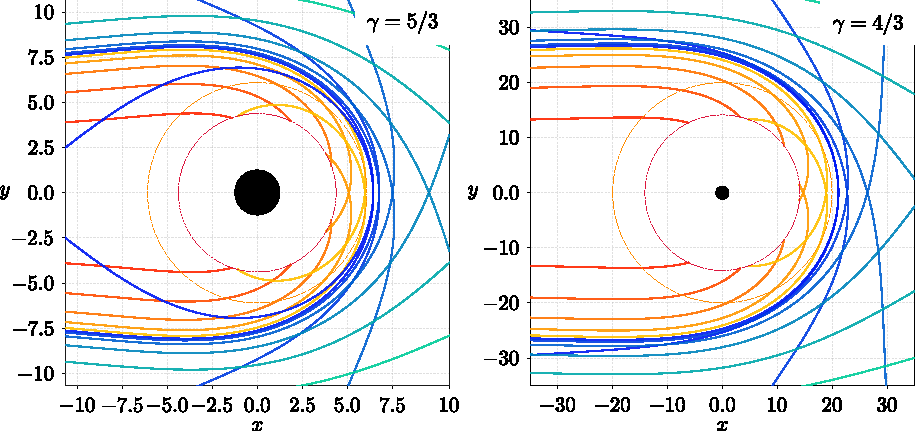
\includegraphics[width=\linewidth]{phonon_orbits_both.pdf}
\caption{Траектории звуковых лучей в течении Мишеля при $a_{\infty}=0{,}1$ для одноатомного газа ($\gamma=5/3$, слева) и радиационно-доминированной плазмы ($\gamma=4/3$, справа). Захватываемые лучи ($b<b_{\mathrm{c}}$) по спирали наматываются на акустический горизонт $r_{\mathrm{a}}$, тогда как рассеиваемые лучи ($b>b_{\mathrm{c}}$) отклоняются, огибая акустическую фотонную сферу $r_{\mathrm{aph}}$.}
\label{fig:phonon-orbits}
\end{figure}

\begin{figure}[p]
\centering
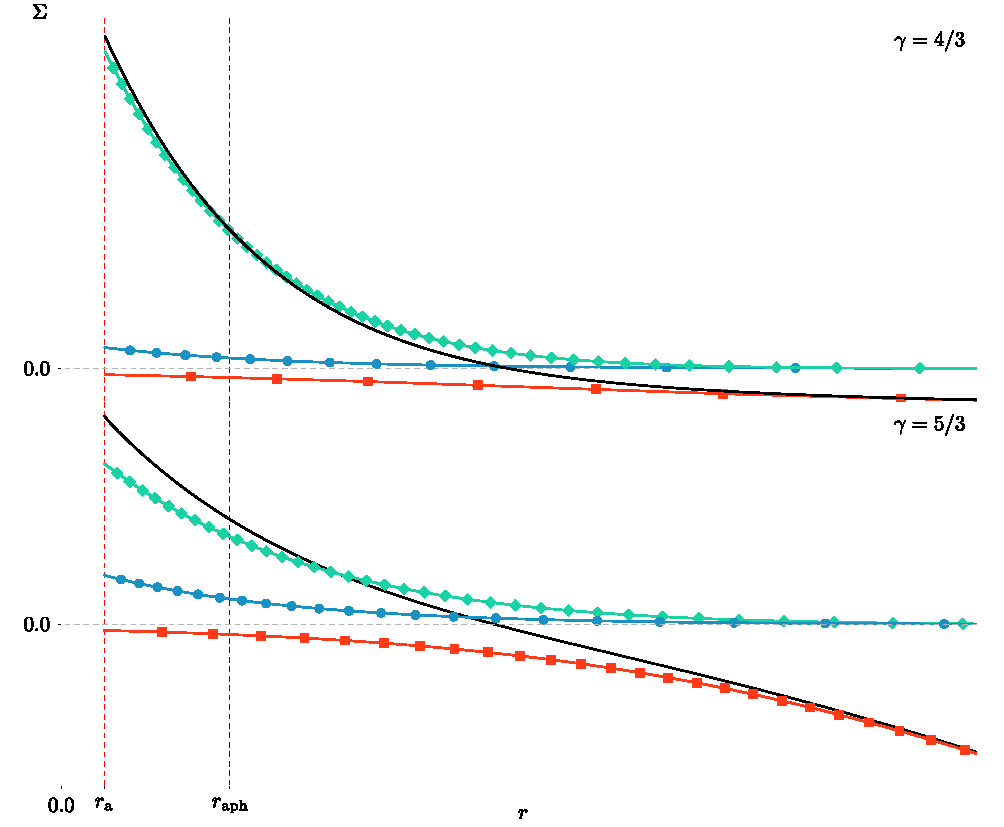
\includegraphics[width=0.8\linewidth]{phonon_forces.pdf}
\caption{Разложение силы~\eqref{eq:binet-second-acoustic} вдоль критического луча $b=b_{\mathrm{c}}$ ($a_{\infty}=0{,}1$) для $\gamma=4/3$ (сверху) и $\gamma=5/3$ (снизу).}
\label{fig:phonon-forces}
\end{figure}

\begin{figure}[p]
\centering
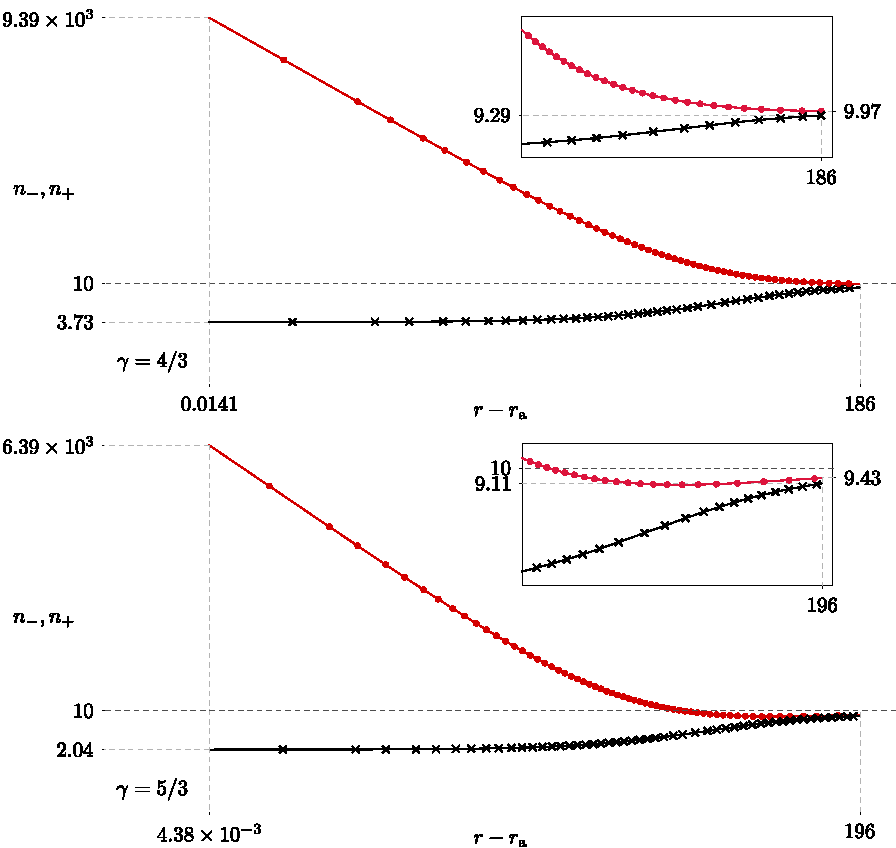
\includegraphics[width=0.75\linewidth]{shapiro_compare.pdf}
\caption{Локальное замедление $n_{\pm}=f/|v_{\pm}|$ для исходящих и входящих лучей ($a_{\infty}=0{,}1$). Вблизи горизонта исходящая ветвь замерзает ($n_{+}\to\infty$), тогда как входящая остаётся конечной.}
\label{fig:shapiro}
\end{figure}

\begin{figure}[p]
\centering
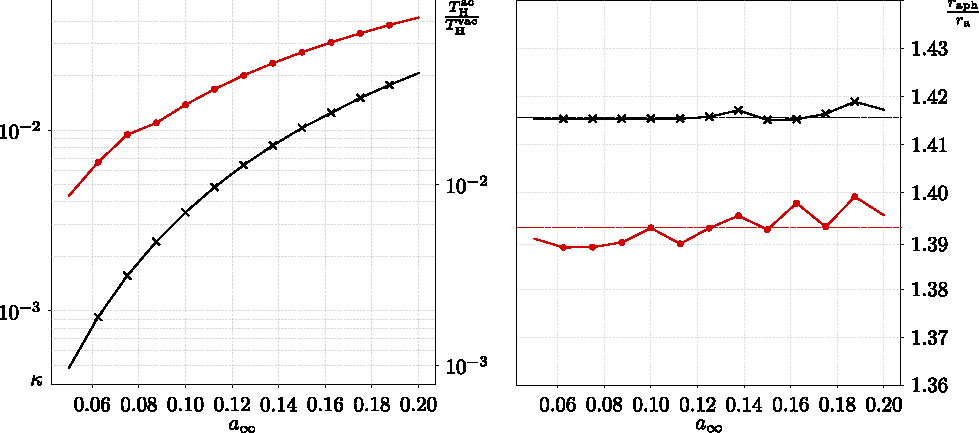
\includegraphics[width=0.88\linewidth]{ainf_scan.pdf}
\caption{Зависимость термодинамики акустического горизонта и геометрии линзирования от асимптотической скорости звука $a_{\infty}$. Отношение $r_{\mathrm{aph}}/r_{\mathrm{a}}$ остаётся почти постоянным.}
\label{fig:ainf-scan}
\end{figure}

\clearpage
\begin{table}[p]
\centering
\caption{Звуковая точка Мишеля (совпадающая с акустическим горизонтом), $r_{\mathrm{a}}=r_{\mathrm{c}}$, и скорость звука $a_{\mathrm{c}}$ в ней.}
\label{tab:sonic-point}
{\small
\begin{tabular}{cccc}
\toprule
$\gamma$ & $a_{\infty}$ & $r_{\mathrm{a}}=r_{\mathrm{c}}$ & $a_{\mathrm{c}}$ \\
\midrule
$4/3$ & $0{,}01$ & $1252$ & $0{,}014$ \\
$4/3$ & $0{,}03$ & $141$  & $0{,}042$ \\
$4/3$ & $0{,}10$ & $14{,}1$ & $0{,}137$ \\
$5/3$ & $0{,}01$ & $38{,}1$ & $0{,}082$ \\
$5/3$ & $0{,}03$ & $13{,}1$ & $0{,}142$ \\
$5/3$ & $0{,}10$ & $4{,}38$ & $0{,}262$ \\
\bottomrule
\end{tabular}
}
\end{table}

\begin{table}[p]
\centering
\caption{Силы $F_{\mathrm{E}}$, $F_{\mathrm{R}}$, $F_{\mathrm{W}}$ из~\eqref{eq:binet-second-acoustic} и их сумма $\Sigma=F_{\mathrm{E}}+F_{\mathrm{R}}-F_{\mathrm{W}}$. $a_{\infty}=0{,}1$.}
\label{tab:phonon-forces}
{\small
\setlength{\tabcolsep}{4.5pt}
\begin{tabular}{llcccccc}
\toprule
$\gamma$ & точка & $r$ & $F_{\mathrm{E}}$ & $F_{\mathrm{R}}$ & $F_{\mathrm{W}}$ & $\Sigma$ & $1/b^{2}_{\mathrm{c}}$ \\
\midrule
\multirow{3}{*}{$5/3$}
  & $r_{\mathrm{a}}$   & $4{,}38$  & $+7{,}81\cdot 10^{-2}$ & $-8{,}95\cdot 10^{-3}$ & $-2{,}55\cdot 10^{-1}$ & $+3{,}24\cdot 10^{-1}$ & \multirow{3}{*}{$4{,}01\cdot 10^{-4}$} \\
  & $r_{\mathrm{aph}}$ & $6{,}10$  & $+4{,}04\cdot 10^{-2}$ & $-1{,}54\cdot 10^{-2}$ & $-1{,}39\cdot 10^{-1}$ & $+1{,}64\cdot 10^{-1}$ & \\
  & $r_{0}$          & $12{,}16$ & $+1{,}01\cdot 10^{-2}$ & $-4{,}49\cdot 10^{-2}$ & $-3{,}47\cdot 10^{-2}$ & $0$ & \\
\midrule
\multirow{3}{*}{$4/3$}
  & $r_{\mathrm{a}}$   & $14{,}11$ & $+7{,}53\cdot 10^{-3}$ & $-2{,}23\cdot 10^{-3}$ & $-1{,}15\cdot 10^{-1}$ & $+1{,}20\cdot 10^{-1}$ & \multirow{3}{*}{$1{,}73\cdot 10^{-5}$} \\
  & $r_{\mathrm{aph}}$ & $19{,}98$ & $+3{,}76\cdot 10^{-3}$ & $-3{,}26\cdot 10^{-3}$ & $-4{,}96\cdot 10^{-2}$ & $+5{,}01\cdot 10^{-2}$ & \\
  & $r_{0}$          & $43{,}41$ & $+7{,}96\cdot 10^{-4}$ & $-6{,}45\cdot 10^{-3}$ & $-5{,}65\cdot 10^{-3}$ & $0$ & \\
\bottomrule
\end{tabular}
}
\end{table}

\begin{table}[p]
\centering
\caption{Интегральные характеристики акустического эффекта Шапиро. $a_{\infty}=0{,}1$.}
\label{tab:shapiro}
{\small
\setlength{\tabcolsep}{4.5pt}
\begin{tabular}{lccccccc}
\toprule
$\gamma$ & $r_{1}/r_{\mathrm{a}}$ & $r_{1}$ & $n_{+}$ & $n_{-}$ & $\Delta t^{\mathrm{ac}}_{+}$ & $R$ & $\mathcal{T}$ \\
\midrule
\multirow{3}{*}{$4/3$}
  & $1{+}10^{-3}$ & $14{,}1$ & $9{,}39\cdot 10^{3}$ & $3{,}73$ & $2813$ & $1035$ & $15{,}9$ \\
  & $1.5$         & $21{,}2$ & $27{,}2$             & $4{,}60$ & $1875$ & $819$  & $11{,}3$ \\
  & $4.0$         & $56{,}4$ & $11{,}7$             & $7{,}12$ & $1357$ & $1062$ & $10{,}4$ \\
\midrule
\multirow{3}{*}{$5/3$}
  & $1{+}10^{-3}$ & $4{,}39$ & $6{,}39\cdot 10^{3}$ & $2{,}04$ & $1902$ & $467$ & $10{,}5$ \\
  & $1.5$         & $6{,}57$ & $20{,}3$             & $2{,}55$ & $1663$ & $465$ & $9{,}42$ \\
  & $4.0$         & $17{,}5$ & $9{,}97$             & $4{,}34$ & $1526$ & $613$ & $9{,}24$ \\
\bottomrule
\end{tabular}
}
\end{table}

\begin{table}[p]
\centering
\caption{Поверхностная гравитация акустического горизонта из~\eqref{eq:surface-gravity-explicit}. $a_{\infty}=0{,}1$.}
\label{tab:surface-gravity}
{\small
\begin{tabular}{ccccc}
\toprule
$\gamma$ & $r_{\mathrm{a}}=r_{\mathrm{c}}$ & $\kappa$ & $T_{\mathrm{H}}=\kappa/2\pi$ & $2\kappa=T^{\mathrm{ac}}_{\mathrm{H}}/T^{\mathrm{vac}}_{\mathrm{H}}$ \\
\midrule
$5/3$   & $4{,}38$  & $1{,}38\cdot 10^{-2}$ & $2{,}20\cdot 10^{-3}$ & $2{,}76\cdot 10^{-2}$ \\
$4/3$   & $14{,}11$ & $3{,}51\cdot 10^{-3}$ & $5{,}58\cdot 10^{-4}$ & $7{,}02\cdot 10^{-3}$ \\
\midrule
вакуум    & $1$     & $1/2$               & $1/4\pi$            & $1$ \\
\bottomrule
\end{tabular}
}
\end{table}

\begin{table}[p]
\centering
\caption{Зависимость от асимптотической скорости звука $a_{\infty}$.}
\label{tab:ainf-scan}
{\small
\begin{tabular}{ccccccc}
\toprule
$\gamma$ & $a_{\infty}$ & $r_{\mathrm{a}}$ & $r_{\mathrm{aph}}$ & $r_{\mathrm{aph}}/r_{\mathrm{a}}$ & $\kappa$ & $2\kappa$ \\
\midrule
\multirow{4}{*}{$5/3$}
  & $0{,}05$ & $8{,}13$ & $11{,}29$ & $1{,}39$ & $4{,}10\cdot 10^{-3}$ & $8{,}20\cdot 10^{-3}$ \\
  & $0{,}10$ & $4{,}38$ & $6{,}10$  & $1{,}39$ & $1{,}38\cdot 10^{-2}$ & $2{,}76\cdot 10^{-2}$ \\
  & $0{,}15$ & $3{,}14$ & $4{,}37$  & $1{,}39$ & $2{,}69\cdot 10^{-2}$ & $5{,}39\cdot 10^{-2}$ \\
  & $0{,}20$ & $2{,}51$ & $3{,}52$  & $1{,}40$ & $4{,}19\cdot 10^{-2}$ & $8{,}39\cdot 10^{-2}$ \\
\midrule
\multirow{4}{*}{$4/3$}
  & $0{,}05$ & $51{,}67$ & $73{,}13$ & $1{,}42$ & $4{,}82\cdot 10^{-4}$ & $9{,}64\cdot 10^{-4}$ \\
  & $0{,}10$ & $14{,}11$ & $19{,}97$ & $1{,}42$ & $3{,}51\cdot 10^{-3}$ & $7{,}02\cdot 10^{-3}$ \\
  & $0{,}15$ & $7{,}10$  & $10{,}06$ & $1{,}42$ & $1{,}03\cdot 10^{-2}$ & $2{,}06\cdot 10^{-2}$ \\
  & $0{,}20$ & $4{,}60$  & $6{,}51$  & $1{,}42$ & $2{,}06\cdot 10^{-2}$ & $4{,}13\cdot 10^{-2}$ \\
\bottomrule
\end{tabular}
}
\end{table}

\clearpage
\bibliographystyle{elsarticle-num}
\bibliography{article}

\end{document}